\chapter{Confronto dei metodi di despeckling}
Per ogni approccio utilizzato è stato calcolato sia il PSNR che SSIM, in modo da capire 
quanto bene è stato eseguito il despeckling e come è 
stata mantenuta la struttura dell'immagine in relazione anche ai modelli di base che sono stati fusi.

\section{Metriche per la valutazione delle immagini despeckled}
\subsection{Peak Signal-to-Noise Ratio}
Per la valutazione della qualità delle immagini despeckled è stata utilizzata la metrica PSNR come indicatore.
Il PSNR è una metrica usata per misurare la qualità di un’immagine ricostruita o 
compressa rispetto a un’immagine di riferimento (ground truth). 
Si basa sull’errore quadratico medio (MSE, Mean Squared Error) tra i pixel dell’immagine originale e 
quelli dell’immagine degradate/ricostruita. La formuala è: 
\begin{equation}
  \makebox[\textwidth][c]{%
    $\displaystyle
    \text{PSNR} = 10 \cdot \log_{10} \left( \frac{MAX_I^2}{\text{MSE}} \right)
    $%
  }
\end{equation}
Dove $MAX_I$ è il valore massimo possibile per un pixel. Più alto è il PSNR, migliore è la qualità dell’immagine ricostruita.
\subsection{Structural Similarity Index}
Un’altra metrica utilizzata per la valutazione della qualità delle immagini despeckled è lo SSIM. 
SSIM è progettato per valutare la qualità percepita di un’immagine rispetto a un’immagine di riferimento, 
tenendo conto delle caratteristiche strutturali dell’immagine. La formula è:
\begin{equation}
  \makebox[\textwidth][c]{%
    $\displaystyle
    \text{SSIM}(x, y) = \frac{(2\mu_x \mu_y + C_1)(2\sigma_{xy} + C_2)}{(\mu_x^2 + \mu_y^2 + C_1)(\sigma_x^2 + \sigma_y^2 + C_2)}
    $%
  }
\end{equation}
Dove:
\begin{itemize}
  \item $\mu_x$ e $\mu_y$ sono le medie delle immagini x e y.
  \item $\sigma_x^2$ e $\sigma_y^2$ sono le varianze delle immagini x e y.
  \item $\sigma_{xy}$ è la covarianza tra le immagini x e y.
  \item $C_1$ e $C_2$ sono costanti per stabilizzare la divisione quando i denominatori sono piccoli.   
\end{itemize}


\subsection{Tabella di confronto tramite PSNR della media e media pesata}
\begin{table}[H] % ambiente table per inserire una didascalia
  \centering
  \resizebox{1.0\textwidth}{!}{% <-- qui scegli quanto ridurla (0.9 = 90%)
    \begin{tabular}{|c|c|c|c|c|c|c|}
    \hline
    Bioma & SAR-CAM & FANS & SARBM3D & MEDIA & MEDIA PESATA \\ \hline
    Agricultural &  24.95  & 24.58  & 25.37 & 25.28 & 25.29 \\ \hline
    Airplane & 26.07 & 23.91 & 23.20 & 24.85 & 24.77 \\ \hline
    Chaparral & 22.93 & 21.49 & 22.43 & 22.60 & 22.59  \\ \hline
    Harbor & 23.17 & 21.09 & 20.56 & 22.13 & 22.08  \\ \hline
    \end{tabular}
  } % fine resizebox
  \caption{Confronto dei modelli di despeckling e della loro fusione. 
            I valori sopra, indicano la media del PSNR di 100 immagini rappresentanti diversi biomi.
            Ogni modello per la previsione della qualità, usato in MEDIA PESATA, 
            è stato allenato per 10 epoche con un dataset da 30'000 
            immagini. }
  \label{tab:valoriPSNR_MN_MP}
\end{table}    
Dall’analisi dei valori di PSNR riportati in Tabella \ref{tab:valoriPSNR_MN_MP}, è possibile osservare che i metodi di fusione 
MEDIA e MEDIA PESATA si comportano in modo coerente rispetto alle prestazioni dei singoli modelli di despeckling (SAR-CAM, FANS e SARBM3D). 
In generale, i valori di MEDIA e MEDIA PESATA risultano compresi tra quelli dei tre modelli originari, come atteso da una procedura di 
fusione. Questo comportamento indica che la combinazione delle uscite tende ad attenuare le debolezze dei singoli modelli, garantendo una 
maggiore stabilità e robustezza complessiva del risultato.
Nella maggior parte dei biomi considerati, la MEDIA raggiunge valori di PSNR molto vicini al modello con le migliori prestazioni, spesso SARCAM e 
supera nettamente il modello peggiore (solitamente SARBM3D). Ciò dimostra che la fusione aritmetica costituisce una strategia efficace per 
ottenere un risultato medio-bilanciato, in grado di avvicinarsi alla qualità del modello più performante senza sacrificare la coerenza tra le varie scene.
Il confronto tra MEDIA e MEDIA PESATA mostra differenze minime, generalmente inferiori a 0.05 dB su tutto il dataset. Tale scostamento 
marginale suggerisce che i pesi adottati nella media pesata non hanno inciso in modo significativo sul risultato finale, probabilmente a 
causa di una distribuzione dei pesi simile a quella uniforme o di prestazioni già bilanciate tra i tre modelli di base.
Nel complesso, la fusione dei risultati anche nella sua forma più semplice permette di ottenere un compromesso ottimale tra i diversi 
approcci di despeckling, mantenendo un livello di qualità molto vicino al migliore modello individuale e al contempo più 
stabile rispetto alle variazioni del contenuto dell’immagine. Tuttavia non riesce nella maggior parte dei casi a dare 
risultati migliori rispetto al miglior modello.

\subsection{Tabella di confronto tramite SSIM della media e della media pesata}
\begin{table}[H] % ambiente table per inserire una didascalia
    \centering
    \resizebox{1.0\textwidth}{!}{% <-- qui scegli quanto ridurla (0.9 = 90%)
      \begin{tabular}{|c|c|c|c|c|c|c|}
      \hline
      Bioma & SAR-CAM & FANS & SARBM3D & MEDIA & MEDIA PESATA \\ \hline
      Agricultural & 0.55 & 0.47 & 0.59 & 0.55 & 0.55  \\ \hline
      Airplane & 0.71 & 0.67 & 0.68 & 0.70 & 0.70  \\ \hline
      Chaparral & 0.62 & 0.46 & 0.56 & 0.57 & 0.57 \\ \hline
      Harbor & 0.81 & 0.74 & 0.74 & 0.78 & 0.78 \\ \hline
      \end{tabular}
    } % fine resizebox
    \caption{Confronto dei modelli di despeckling e della loro fusione. 
              I valori sopra, indicano la media del SSIM di 100 immagini rappresentanti diversi biomi.
              Ogni modello per la previsione della qualità, usato in MEDIA PESATA, 
              è stato allenato per 10 epoche con un dataset da 30'000 
              immagini. }
    \label{tab:valoriSSIM_MN_MP}
  \end{table}  
  Anche dai dati riportati nella tabella \ref{tab:valoriSSIM_MN_MP} si osserva come sia la MEDIA sia la MEDIA PESATA 
  tendano a riflettere le prestazioni del modello migliore in termini di SSIM. La qualità strutturale dell’immagine 
  non risulta mai inferiore o pari a quella del modello meno performante, confermando che, sebbene questo 
  approccio non rappresenti la soluzione ottimale, costituisce comunque un buon compromesso tra i diversi modelli.
  \subsubsection{Tabella di confronto tramite PSNR del modello crossfuse}
  \begin{table}[H] % ambiente table per inserire una didascalia
    \centering
    \resizebox{1.0\textwidth}{!}{% <-- qui scegli quanto ridurla (0.9 = 90%)
      \begin{tabular}{|c|c|c|c|c|c|c|}
      \hline
      Bioma & SAR-CAM & FANS & SARBM3D & CROSSFUSE & CROSSFUSE LIGHT \\ \hline
      Agricultural &  24.95  & 24.58  & 25.37 &  & 23.73 \\ \hline
      Airplane & 26.07 & 23.91 & 23.20 &  & 26.48  \\ \hline
      Chaparral & 22.93 & 21.49 & 22.43 &  &  21.90 \\ \hline
      Harbor & 23.17 & 21.09 & 20.56 &  & 22.28 \\ \hline
      \end{tabular}
    } % fine resizebox
    \caption{Confronto dei modelli di despeckling e della loro fusione tramite CrossFuse tramite PSNR.}
    \label{tab:valoriPSNR_CF_TN}
  \end{table}     
  \subsubsection{Tabella di confronto tramite SSIM del modello crossfuse}
  \begin{table}[H] % ambiente table per inserire una didascalia
    \centering
    \resizebox{1.0\textwidth}{!}{% <-- qui scegli quanto ridurla (0.9 = 90%)
      \begin{tabular}{|c|c|c|c|c|c|c|}
      \hline
      Bioma & SAR-CAM & FANS & SARBM3D & CROSSFUSE & CROSSFUSE LIGHT \\ \hline
      Agricultural & 0.55 & 0.47 & 0.59 & 0.38 &  0.54 \\ \hline
      Airplane & 0.71 & 0.67 & 0.68 & 0.45 & 0.70  \\ \hline
      Chaparral & 0.62 & 0.46 & 0.56 & 0.48 & 0.62 \\ \hline
      Harbor & 0.81 & 0.74 & 0.74 & 0.64 & 0.78 \\ \hline
      \end{tabular}
    } % fine resizebox
    \caption{Confronto dei modelli di despeckling e della loro fusione tramite CrossFuse tramite SSIM.}
    \label{tab:valoriSSIM_MN_MP}
  \end{table}     
  QUI METTERE LE CONSIDERAZIONI UNA VOLTA VISTI I RISULTATI  

  \subsection{Confronto visivo dei vari modelli}
  \subsubsection{Media pesata}
  \begin{figure}[H]
    \centering
    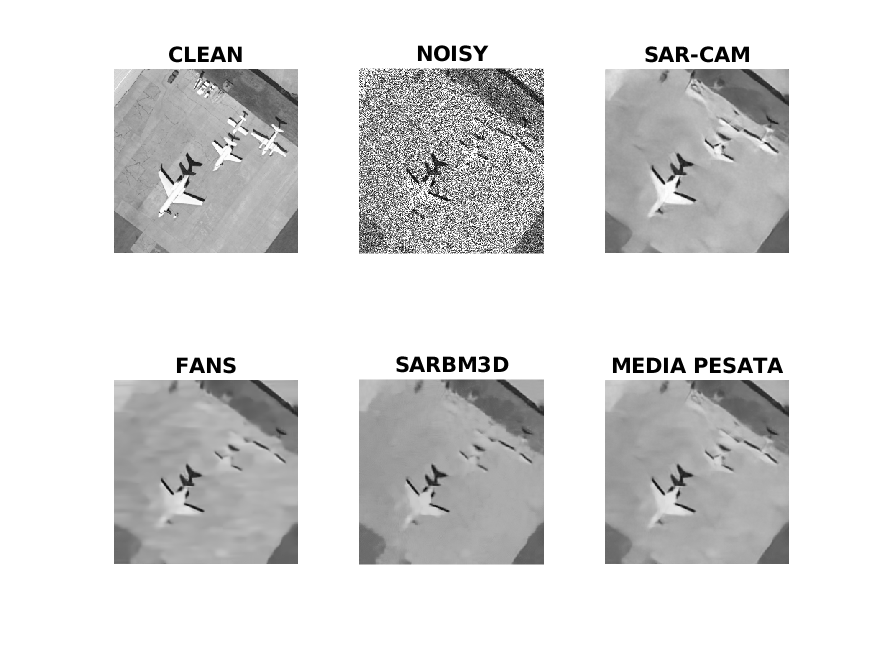
\includegraphics[width=1.1\textwidth]{utils/MPairplane00.png}
    \caption{}
    \label{fig:airplane00MP}
  \end{figure}
Confrontando i singoli modelli di despeckling con il ground truth si puo notare come sia SARBM3D che FANS abbiano 
perso dettagli sematici importanti durante il denoising come ad esempio l'aero più piccolo e il corpo principale degli aerei accanto sono spariti dall'immagine despeckled.
SARCAM invece preserva meglio le informazioni semantiche eseguendo un despeckling che si avvicina di più all'immagine clean.
Nell'immagine con i tre modelli fusi tramite la media pesata notiamo che sono stati riportati gli aerei che si erano persi in FANS e SARBM3D. 
Cio torna con l'analisi fatta con le metriche come PSNR e SSIM in cui l'immagine fusa tende sempre ad allinearsi al modello migliore senza fare mai 
peggio del modello meno efficace.
\subsubsection{media aritmetica}
\begin{figure}[H]
    \centering
    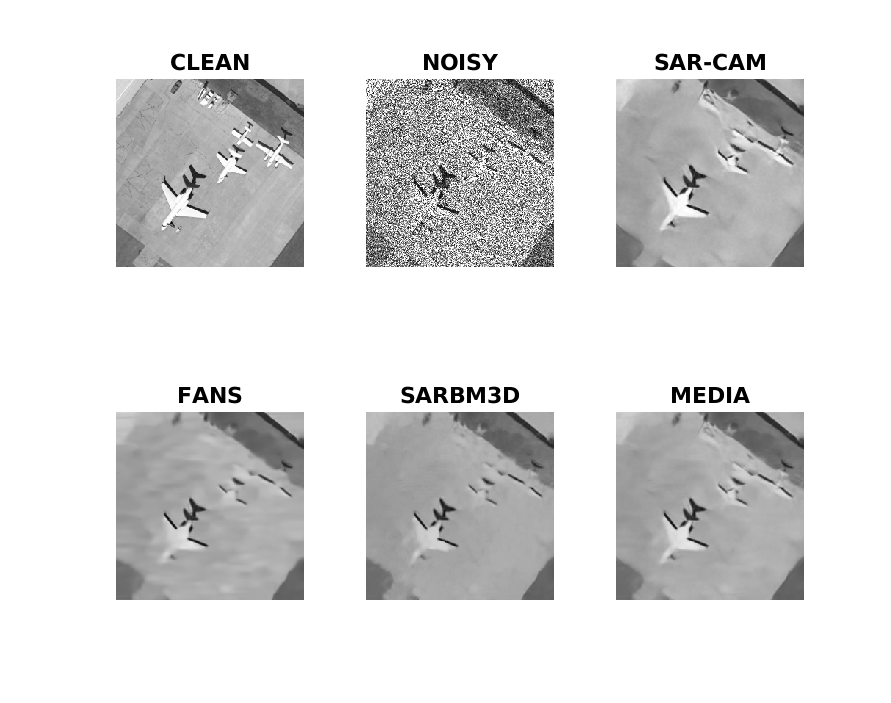
\includegraphics[width=1.1\textwidth]{utils/MNairplane00.png}
    \caption{}
    \label{fig:airplane00MN}
  \end{figure}
  Queste immagini ci danno la prova visiva di quanto già osservato attraverso le metriche PSNR e SSIM, ovvero che 
  la media aritmetica si comporta in modo molto simile alla media pesata. In entrambi i casi, la fusione tende a 
  privilegiare le regioni in cui i singoli modelli hanno performato meglio, combinando in maniera efficace le 
  loro rispettive capacità di riduzione del rumore e preservazione del dettaglio.